\subsection{Processo, processo sw, modello di processo, elementi caratteristici dei processi}
\begin{itemize}
    \item Processo:Un insieme coerente di attività per specificazione, progettazione, implementazione e testing di sistemi software.
    \item processo software: Un insieme strutturato di attività necessarie per sviluppare un sistema software
    \item modello di processo software: è una rappresentazione astratta di un processo che presenta una descrizione da una prospettiva particolare.
    \item Elementi caratteristici dei processi:
    \begin{description}
        \item[Input] ciò che il processo considera come punto di partenza, da trasformare nei risultati dell'esecuzione del processo
        \item[Prodotti o output] quali sono i risultati di un'attività di processo
        \item[Ruoli] che riflettono le responsabilità delle persone coinvolte nel processo
        \item[Risorse] necessario per l'esecuzione del processo
        \item[Pre/Post condizione] che sono affermazioni vere prima e dopo l'attivazione di un'attività di processo o la produzione di un prodotto.
    \end{description}
\end{itemize}
\subsection{Processi plan-driven, processi agili}
\begin{itemize}
    \item \textit{plan-driven}: sono processi dove tutti i processi sono pianificati \textbf{in anticipo} e il progresso è misurato rispetto al piano.
    \item Nei processi agili, la pianificazione è incrementale ed è più semplice modificare il processo per riflettere le mutevoli esigenze dei clienti.
    \item in pratica, la maggior parte dei processi pratici include elementi sia dai \textit{plan-driven} che dagli approcci agili.
\end{itemize}
\subsection{Waterfall Model, caratteristiche, pregi, criticità}
\begin{itemize}
    \item In un modello a cascata, ogni fase deve essere completata prima che possa iniziare la fase successiva e non vi sono sovrapposizioni nelle fasi che sono:
    \begin{itemize}
        \item definizione dei requisiti
        \item system design
        \item implementazione e unit testing
        \item integrazione e testing del sistema
        \item \textit{deployment}
        \item oparatività e manutenzione
    \end{itemize}
    \item Pregi: gode di una buona visibilità e gestibilità dovuta al fatto che nel passaggio da una fase alla successiva corrisponde la stesura di un documento (analisi dei requisiti, di progetto, di sorgenti, di rapporto tecnico\dots) consegnato e accettato dal committente.
    \item Criticità: La suddivisione non flessibile del progetto in fasi distinte rende difficile rispondere alle mutevoli esigenze dei clienti
\end{itemize}
\subsection{Prototyping/evolutionary development: exploratory prototyping, throw-away prototyping; ciclo iterativo del prototyping; vantaggi, criticità e applicabilità}
\begin{itemize}
    \item \textit{prototyping} si costruiscono e si valuta diverse versioni successive del sistema, al fine di avere più informazioni ed idee sul risultato finale che si vuole ottenere e sul come ottenerlo. Il Sistema può essere di ‘dimensione reali’ o ‘in scala ridotta’.
    \item l'\textit{evolutionary development} si divide in:
    \begin{description}
        \item[exploratory development/prototyping] l'obiettivo è lavorare con i clienti e far evolvere un sistema finale da una specifica di struttura iniziale. Dovrebbe iniziare con requisiti ben compresi, iniziando con ciò che è chiaro e cercando di capire il resto.
        \item[throw-away prototyping] L'obiettivo è comprendere i requisiti di sistema. Dovrebbe iniziare con requisiti poco compresi. Un prototipo viene sviluppato "veloce e sporco", quindi, quando i requisiti sono stati compresi, il prototipo viene gettato via. Concentrando solo su ciò che non è chiaro, al fine di capirlo meglio.
    \end{description}
    \item il modello \textit{evolutionary} è suddiviso nelle seguenti fasi:
    \begin{itemize}
        \item specifica
        \item sviluppo (che produce un prototipo)
        \item validazione
    \end{itemize}
    che possono essere ripetuti più volte, fino al completamento del sistema.
    \item vantaggi:
    \begin{itemize}
        \item riduzione dei costi implementativi se i requisiti cambiano
        \item più feedback dal client
    \end{itemize}
    \item criticità
    \begin{itemize}
        \item mancanza di visibilità
        \item sistemi spesso mal strutturati
        \item possono essere richieste abilità particolari (e.g. in linguaggi per la rapida prototipizzazione)
    \end{itemize}
    \item applicabilità
    \begin{itemize}
        \item per piccoli/medi sistemi interattivi
        \item per tecnologie e sistemi innovativi
        \item per parti di un grande sistema (e.g. user interface)
        \item per sistemi con una breve durata di vita
    \end{itemize}
\end{itemize}
\subsection{Modelli IBRIDI}
Sono modelli che integrano più aspetti insieme.  Ad esempio, il modello waterfall integrato con il prototyping è un waterfall dove allo stadio del sistem testing è possibile tornare indietro all'analisi dei requisiti o al design del sistema.
\subsection{Formal system development: l’idea e i suoi limiti}
È una metodologia che si basa su una serie di trasformazioni di una specifica espressa in linguaggio matematico per giungere a un programma eseguibile.  Si tratta di un processo incrementale che a ogni step viene provato essere corretto.  Si tratta di un modello di scarso utilizzo pratico.
\subsection{Sviluppo basato sul ri-uso: strutturazione in fasi}
Basato sull'idea del riuso sistematico dove il sistema viene integrato da componenti esistenti o COTS (\textit{commercial off-the-shelf}).

Fasi del processo:
\begin{enumerate}
    \item Analisi dei componenti
    \item Modifica dei requisiti
    \item Progettazione del sistema con riutilizzo
    \item Sviluppo e integrazione
\end{enumerate}

\subsection{Cicli di Processo, iterazione; sviluppo incrementale, incrementi, vantaggi e criticità; sviluppo iterativo}
\begin{itemize}
    \item I requisiti di sistema sono \textbf{sempre in cambiamento} nel corso di un progetto.

    Ci sono due approcci collegati:
    \begin{itemize}
        \item Sviluppo incrementale, e la sua variante denominata Sviluppo iterativo
        \item Sviluppo a spirale
    \end{itemize}
    
    \item Sviluppo incrementale:
    \begin{itemize}
        \item Combina il Waterfall con il modello evolutivo
        \item Lo sviluppo e il rilascio è diviso in \textbf{incrementi} ognuno con una parte delle funzionalità richieste
        \item I requisiti utente sono prioritari e i requisiti di massima priorità sono inclusi nei primi incrementi
        \item Una volta avviato lo sviluppo di un incremento, i requisiti vengono congelati sebbene i requisiti e gli incrementi successivi possano continuare ad evolversi
    \end{itemize}
    
    \item vantaggi:
    \begin{itemize}
        \item Le funzionalità vengono consegnate incrementalmente con ogni rilascio quindi le funzionalità sono disponibili prima: non si deve attendere il completamento di tutto il sistema.
        \item I primi incrementi fungono da prototipi per aiutare la raccolta dei requisiti per i successivi incrementi
        \item Minor rischio di fallimento generale del progetto
        \item I primi incrementi(che hanno la priorità più alta) sono quelli più testati e più sicuri
    \end{itemize}
    
    \item svantaggi:
    \begin{itemize}
        \item Non avendo specifiche complete all'inizio risulta difficile trovare i \enquote{giusti} incrementi per scomporre il sistema
        \item Difficile identificare servizi comuni (strutture di base)
        \item Può richiedere modelli contrattuali non standard o più contratti successivi
    \end{itemize}
    
    \item Sviluppo iterativo: inizia con il sistema completo, quindi cambia funzionalità/implementazione di ciascun sottosistema con ogni nuova versione
\end{itemize}

\subsection{Extreme programming}
\begin{itemize}
    \item Nuovo approccio allo sviluppo basato sullo sviluppo e sulla fornitura di incrementi di funzionalità molto piccoli
    \item Si affida al costante miglioramento del codice, al coinvolgimento degli utenti nel team di sviluppo e alla programmazione a coppie
\end{itemize}
\subsection{Rischio: definizione e ruolo; cause di fallimento di un progetto sw; Modello di sviluppo a spirale, settori della spirale}
Le cause per le quali un progetto di sviluppo software
\begin{itemize}
    \item Requisiti incompleti o vaghi, conflitti tra gli \textit{stakeholders}
    \item Mancanza di coinvolgimento degli utenti
    \item Mancanza di risorse, skill non sufficienti per il lavoro
    \item Aspettative non realistiche
    \item Cattiva gestione del progetto, pianificazione o stima dei costi
    \item Scarso supporto esecutivo
    \item Mancanza di comunicazione
    \item Modifica dei requisiti e delle specifiche
    \item Scarsa architettura
    \item Rilevamento di segnali di avviso di guasto ritardato
\end{itemize}

Il modello a spirale:
\begin{itemize}
    \item Il processo è rappresentato come una spirale piuttosto che come una sequenza di attività con backtracking
    \item Ogni ciclo nella spirale rappresenta una fase del processo.
    \item Nessuna fase fissa come specifica o design - i loop nella spirale sono scelti a seconda di ciò che è richiesto
    \item I rischi vengono esplicitamente valutati e risolti durante l'intero processo
    \item Si parte dalle attività che hanno il più alto livello di rischio.
\end{itemize}
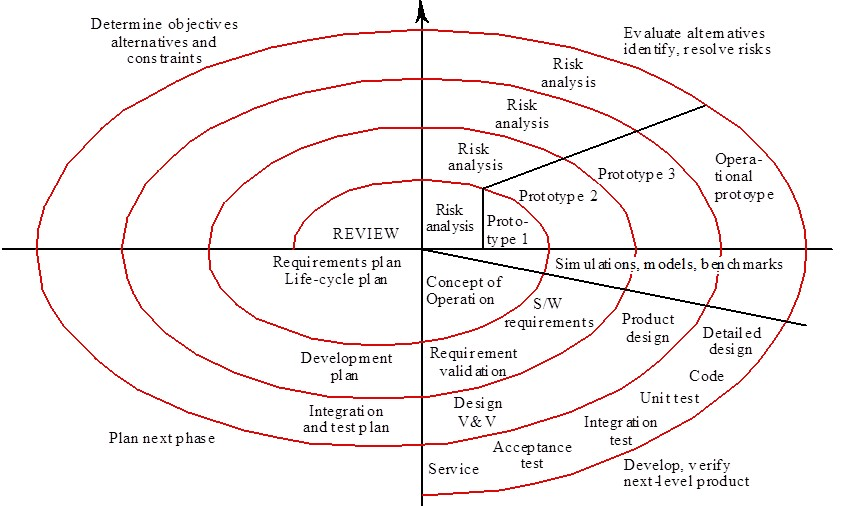
\includegraphics[width=\textwidth]{spirale.jpg}

Settori della spirale:
\begin{itemize}
    \item Definizione degli obiettivi: vengono identificati obiettivi specifici per la fase
    \item Valutazione e riduzione del rischio: vengono valutati i rischi e vengono messe in atto attività per ridurre i rischi chiave
    \item Sviluppo e validazione: viene scelto un modello di sviluppo per il sistema che può essere uno qualsiasi dei modelli generici
    \item Pianificazione: il progetto viene rivisto e viene pianificata la fase successiva della spirale
\end{itemize}
\subsection{Attività fondamentali dei processi primari per lo sviluppo del sw}
\begin{description}
    \item[\red{Analisi dei requisiti} e \blue{specifiche sw}] \red{Il processo di analisi delle esigenze} e \blue{di determinazione dei servizi richiesti e dei vincoli} per il funzionamento e lo sviluppo del sistema. Studio di fattibilità, Richiamo e analisi dei requisiti, Specifica dei requisiti e Convalida dei requisiti
    \item[Progettazione e realizzazione] Il processo di conversione delle specifiche di sistema in un sistema eseguibile. Le attività di progettazione e realizzazione sono strettamente correlate e possono essere interrelate.
    \item[Validazione] \red{La verifica} e \blue{la convalida} hanno lo scopo di dimostrare che un sistema \red{è conforme alle sue specifiche} e \blue{soddisfa realmente le esigenze e i requisiti del cliente del sistema}
    \item[Evoluzione] Il software è intrinsecamente flessibile e può cambiare. Poiché i requisiti cambiano in base alle mutevoli circostanze aziendali, anche il software che supporta l'azienda deve evolversi e cambiare. Sebbene ci sia stata una delimitazione tra sviluppo ed evoluzione (manutenzione), ciò è sempre più irrilevante in quanto sempre meno sistemi sono completamente nuovi
\end{description}
\subsection{Definizione di CASE, varietà delle funzionalità e copertura dell’intero ciclo di vita}
\begin{description}
    \item[CASE] Computer-aided software engineering è un software a supporto dello sviluppo del software e dei processi di evoluzione
\end{description}